%************************************************
\section{helloworld.tex}
\begin{frame}\frametitle{准备工作}
    \begin{itemize}
        \item TEX套装
            \begin{itemize}
        		\item Windows:MiKTeX, \textcolor{red}{CTeX}
        		\item Linux:teTEX
        		\item 跨平台:\textcolor{red}{TeX Live}, MacTeX, ConTeXt
        	\end{itemize}
        \item 编译器
            \begin{itemize}
        		\item Windows:TeXnicCenter, MeWa, WinShell, BakoMa TeX, Inlage, \textcolor{red}{WinEdt}, \ldots
        		\item Linux:Gedit LaTeX Plugin, Gummi, Winefish, \textcolor{red}{Kile}, \ldots
        		\item 跨平台:\textcolor{red}{LyX}, Texmaker, AUCTEX, TeXlipse, \textcolor{red}{TeXworks}, \ldots
        		\item 详细比较:\\http://en.wikipedia.org/wiki/Comparison\_of\_TeX\_editors
        		\item vim和emacs可以通过相应插件来支持\LaTeX
        	\end{itemize}
    \end{itemize}
\end{frame}

\begin{frame}\frametitle{编译过程}
    \begin{figure}[t]
        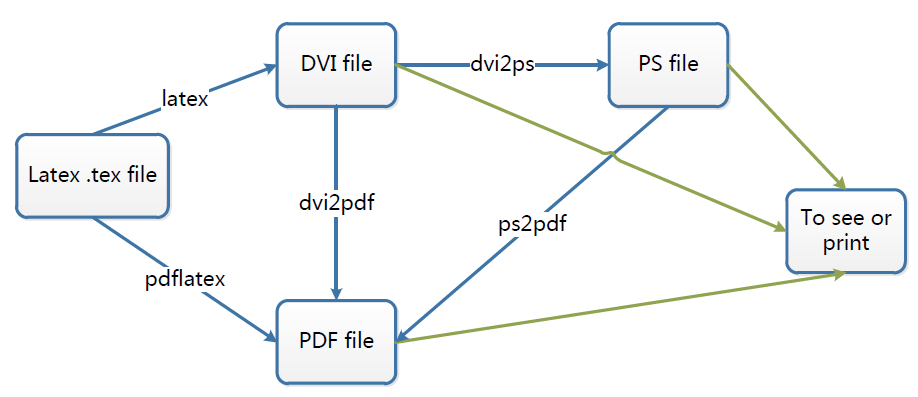
\includegraphics[width=0.8\textwidth]{compile_procedure.png}
    \end{figure}
    \begin{block}{}
        \center
      其中DVI、PostScript和PDF为三种输出格式。
    \end{block}
\end{frame}



\begin{frame}[fragile]
\frametitle{动手写一个hello \LaTeX{}}
    \begin{block}{HelloLatex.tex}
    \begin{verbatim}
% !Mode:: "TeX:UTF-8"
\documentclass{article}
\author{fool}
\title{My First \LaTeX{} article}

\begin{document}
\maketitle
    Wow! This is my FIRST \LaTeX{} Article!

    Hello World!
\end{document}
    \end{verbatim}
    \end{block}
\end{frame}

\begin{frame}[fragile]\frametitle{基本语法介绍}
    \begin{itemize}
        \hidark<1> \item 空格:连续的空格被认为只有一个,用\verb|~|表示空格
        \hidark<2> \item 有些特殊的符号是不能直接使用的:\\
                    \verb|$ & % # _ { }|
                    应该写成
                    \verb|\$ \& \% \# \_ \{ \}|
        \hidark<3> \item 断行:\verb|\\|
        \hidark<4> \item 分段:文字之后的一个空行是段落结束的标志
        \hidark<5> \item 注释:\verb|%|之后都文字都是注释,是无效的语句
        \hidark<6> \item LaTeX的命令:以\verb|\|开始: \\
                    \begin{verbatim}
    \section{第一段}
    \emph{强调}
                   \end{verbatim}
    \end{itemize}
\end{frame}